\let\negmedspace\undefined
\let\negthickspace\undefined
\documentclass[journal,12pt,onecolumn]{IEEEtran}
\usepackage{cite}
\usepackage{amsmath,amssymb,amsfonts,amsthm}
\usepackage{algorithmic}
\usepackage{graphicx}
\graphicspath{{./figs/}}
\usepackage{textcomp}
\usepackage{xcolor}
\usepackage{txfonts}
\usepackage{listings}
\usepackage{enumitem}
\usepackage{mathtools}
\usepackage{gensymb}
\usepackage{comment}
\usepackage{caption}
\usepackage[breaklinks=true]{hyperref}
\usepackage{tkz-euclide} 
\usepackage{listings}
\usepackage{gvv}                                        
%\def\inputGnumericTable{}                                 
\usepackage[latin1]{inputenc}     
\usepackage{xparse}
\usepackage{color}                                            
\usepackage{array}                                            
\usepackage{longtable}                                       
\usepackage{calc}                                             
\usepackage{multirow}
\usepackage{multicol}
\usepackage{hhline}                                           
\usepackage{ifthen}                                           
\usepackage{lscape}
\usepackage{tabularx}
\usepackage{array}
\usepackage{float}
\newtheorem{theorem}{Theorem}[section]
\newtheorem{problem}{Problem}
\newtheorem{proposition}{Proposition}[section]
\newtheorem{lemma}{Lemma}[section]
\newtheorem{corollary}[theorem]{Corollary}
\newtheorem{example}{Example}[section]
\newtheorem{definition}[problem]{Definition}
\newcommand{\BEQA}{\begin{eqnarray}}
\newcommand{\EEQA}{\end{eqnarray}}
\newcommand{\define}{\stackrel{\triangle}{=}}
\theoremstyle{remark}
\newtheorem{rem}{Remark}
\newcommand{\brak}[1]{\left[ #1 \right]}


\begin{document}

\title{
ASSIGNMENT 2: GATE 2012\\
GG : Geology and Geophysics}
\author{EE25BTECH11003 -Adharvan Kshathriya Bommagani}
\maketitle
\renewcommand{\thefigure}{\theenumi}
\renewcommand{\thetable}

\begin{align*}
    {\large{\textbf{PART A: COMMON TO BOTH GEOLOGY AND GEOPHYSICS CANDIDATES}}}
\end{align*}

\subsection*{Q.\ 1 -- Q.\ 25 carry one mark each.}

\begin{enumerate}

\item In Mohs' scale of hardness, how many minerals are of silicate composition?

\hfill{\brak{\text{GATE GG 2012}}}

\begin{multicols}{4}
\begin{enumerate}
\item 4
\item 5
\item 6
\item 7
\end{enumerate}
\end{multicols}

\item Which one of the following river systems forms the largest fluvio-deltaic system in the world?

\hfill{\brak{\text{GATE GG 2012}}}

\begin{multicols}{2}
\begin{enumerate}
\item Mississippi--Ohio
\item Red--Mekong
\item Ganga--Brahmaputra
\item Yellow--Ba Hoi
\end{enumerate}
\end{multicols}

\item Which one amongst the following rocks commonly has highest unconfined compressive strength?

\hfill{\brak{\text{GATE GG 2012}}}

\begin{multicols}{2}
\begin{enumerate}
\item Coarse-grained sandstone
\item Mica schist
\item Fossiliferous limestone
\item Massive basalt
\end{enumerate}
\end{multicols}

\item Eparchean unconformity separates geological units of

\hfill{\brak{\text{GATE GG 2012}}}

\begin{multicols}{2}
\begin{enumerate}
\item early Archaean from late Archaean
\item Archaean from Proterozoic
\item Proterozoic from Palaeozoic
\item Archaean from Phanerozoic
\end{enumerate}
\end{multicols}

\item Point bar deposit is associated with

\hfill{\brak{\text{GATE GG 2012}}}

\begin{multicols}{2}
\begin{enumerate}
\item braided river
\item estuary
\item meandering river
\item beach
\end{enumerate}
\end{multicols}

\item Polymetallic nodules on the ocean floor contain significant amounts of:

\hfill{\brak{\text{GATE GG 2012}}}

\begin{multicols}{4}
\begin{enumerate}
\item Cu--Ni--Co
\item Pb--Zn--Ti
\item Hg--Mo--Pt
\item U--Th--Nb
\end{enumerate}
\end{multicols}

\item If the rake of net slip of an inclined fault is $90^\circ$, the fault is

\hfill{\brak{\text{GATE GG 2012}}}

\begin{multicols}{2}
\begin{enumerate}
\item strike-slip fault
\item dip-slip fault
\item oblique-slip fault
\item transcurrent fault
\end{enumerate}
\end{multicols}



\item On a photo-scale of 1:40000, a square shaped open cast coal mine of $1~\text{km}^2$ area would have an area \brak{\text{in cm$^2$}}

\hfill{\brak{\text{GATE GG 2012}}}

\begin{multicols}{4}
\begin{enumerate}
\item 2.50
\item 4.00
\item 6.25
\item 12.00
\end{enumerate}
\end{multicols}

\item Bouguer correction is applied to correct for the gravity anomaly due to mass between station location and

\hfill{\brak{\text{GATE GG 2012}}}

\begin{multicols}{2}
\begin{enumerate}
\item mean sea level
\item local datum plane
\item base of upper crust
\item Mohorovi\v{c}i\'{c} discontinuity
\end{enumerate}
\end{multicols}

\item Which one of the following can be estimated from SP log against a saline-water saturated sandstone formation encountered in a well?

\hfill{\brak{\text{GATE GG 2012}}}

\begin{enumerate}
\item Resistivity of formation water
\item Degree of water saturation
\item Depth of invasion
\item Permeability
\end{enumerate}

\item During its orbital motion around the Sun, the Earth is nearest to the Sun on

\hfill{\brak{\text{GATE GG 2012}}}

\begin{multicols}{4}
\begin{enumerate}
\item March 21
\item July 4
\item September 23
\item January 3
\end{enumerate}
\end{multicols}

\item Which one of the following can be best explored using electromagnetic method?

\hfill{\brak{\text{GATE GG 2012}}}

\begin{enumerate}
\item Oil-bearing strata
\item Coal-bearing strata
\item Disseminated sulphide deposit
\item Massive sulphide deposit
\end{enumerate}

\item Name the planet in the solar system which has its ``day'' longer than its ``year''.

\hfill{\brak{\text{GATE GG 2012}}}

\begin{multicols}{4}
\begin{enumerate}
\item Mercury
\item Venus
\item Mars
\item Neptune
\end{enumerate}
\end{multicols}

\item The most sensitive instrument for magnetic survey is

\hfill{\brak{\text{GATE GG 2012}}}

\begin{enumerate}
\item magnetic field balance
\item fluxgate magnetometer
\item proton precession magnetometer
\item optically pumped magnetometer
\end{enumerate}

\item Which physical property of the medium governs the response of Ground Penetrating Radar \brak{\text{GPR}}?

\hfill{\brak{\text{GATE GG 2012}}}

\begin{enumerate}
\item Electrical conductivity
\item Electromagnetic conductivity
\item Seismic wave velocity
\item Electrical permeability \brak{\text{dielectric permittivity}}
\end{enumerate}

\newpage


\item Out of the following gases which one has the highest contribution towards the greenhouse effect on the Earth?

\hfill{\brak{\text{GATE GG 2012}}}

\begin{multicols}{4}
\begin{enumerate}
\item CO$_2$
\item CO
\item CH$_4$
\item H$_2$O
\end{enumerate}
\end{multicols}

\item Depth range of the `transition zone' associated with phase changes in the Earth's mantle is \brak{\text{in km}}

\hfill{\brak{\text{GATE GG 2012}}}

\begin{multicols}{2}
\begin{enumerate}
\item 35 to 150
\item 150 to 410
\item 410 to 660
\item 660 to 800
\end{enumerate}
\end{multicols}

 \item Choose the correct pair of plutonic rock and its volcanic equivalent.

\hfill{\brak{\text{GATE GG 2012}}}

\begin{multicols}{4}
\begin{enumerate}
\item Gabbro - Trachyte
\item Syenite - Andesite
\item Granite - Rhyolite
\item Granodiorite - Basalt
\end{enumerate} 
\end{multicols}

\item Which of the following is NOT a variety of silica SiO$_2$?

\hfill{\brak{\text{GATE GG 2012}}}

\begin{multicols}{4}
\begin{enumerate}
\item Jasper
\item Coesite
\item Stishovite
\item Flinkite
\end{enumerate}
\end{multicols}

\item Which one of these is NOT a source of sufficient water supply but can transmit certain quantity of water on a regional scale due to leakage?

\hfill{\brak{\text{GATE GG 2012}}}

\begin{multicols}{4}
\begin{enumerate}
\item Aquifer
\item Aquitard
\item Aquiclude
\item Aquifuge
\end{enumerate}
\end{multicols}

\item Identify the type of fault present in the given aerial photograph.

\hfill{\brak{\text{GATE GG 2012}}}



\begin{figure}[H]
\centering
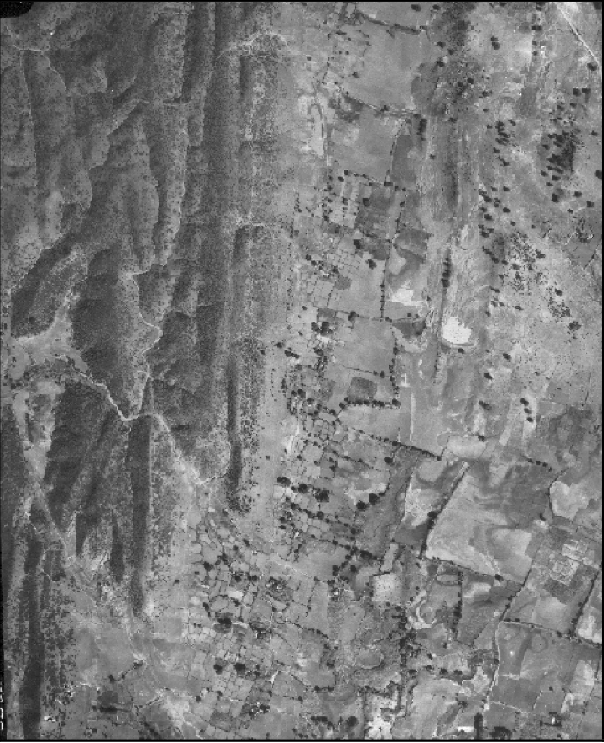
\includegraphics[width=0.7\textwidth]{figs/fig1.png}
\caption{}
\label{fig:q21_fault_photo}
\end{figure}



\begin{multicols}{2}
\begin{enumerate}
\item Normal fault
\item Reverse fault
\item Left\textendash lateral strike\textendash slip fault
\item Right\textendash lateral strike\textendash slip fault
\end{enumerate}
\end{multicols}



\item The Jurassic stratigraphic succession of Kutch is characterized by which one of the following?

\hfill{\brak{\text{GATE GG 2012}}}

\begin{multicols}{4}
\begin{enumerate}
\item Cephalopods
\item Trilobites
\item Brachiopods
\item Graptolites
\end{enumerate}
\end{multicols}

\item Which one of the following mineral constituents exhibits strong absorption in the UV\textendash blue band of the EM spectrum due to charge transfer effect leading to colouration?

\hfill{\brak{\text{GATE GG 2012}}}

\begin{multicols}{4}
\begin{enumerate}
\item Fe\textendash O
\item Si\textendash O
\item Al\textendash OH
\item Mg\textendash OH
\end{enumerate}
\end{multicols}

\newpage

\item When did the supercontinent Pangaea begin to break up?

\hfill{\brak{\text{GATE GG 2012}}}

\begin{multicols}{4}
\begin{enumerate}
\item Cenozoic
\item Mesozoic
\item Palaeozoic
\item Proterozoic
\end{enumerate}
\end{multicols}



\item In which of the following localities does coal deposit occur?

\hfill{\brak{\text{GATE GG 2012}}}

\begin{multicols}{4}
\begin{enumerate}
\item Dariba
\item Kudremukh
\item Wardha
\item Rudrasagar
\end{enumerate}
\end{multicols}

\begin{align*}
    {\large{\textbf{PART B (SECTION 1) FOR GEOLOGY CANDIDATES ONLY}}}
\end{align*}

\subsection*{Q.\ 26 -- Q.\ 55 carry two marks each.}

\item Specific discharge of 1 cm per day is observed in a porous medium where hydraulic head difference is 0.5 m and flow length is 20 m. Calculate the hydraulic conductivity \brak{\text{in m/day}}.

\hfill{\brak{\text{GATE GG 2012}}}

\begin{multicols}{4}
\begin{enumerate}
\item 0.4
\item 0.8
\item 1.2
\item 1.6
\end{enumerate}
\end{multicols}

\item A sandstone bed dipping $30^\circ$ has an outcrop width of 20 m in a flat terrain. What is the true thickness \brak{\text{in m}} of the bed?

\hfill{\brak{\text{GATE GG 2012}}}

\begin{multicols}{4}
\begin{enumerate}
\item 5
\item 10
\item 20
\item 30
\end{enumerate}
\end{multicols}

\item Calculate the concentration \brak{\text{in ppm}} of Ni in olivine that crystallizes from a basaltic magma containing 20 ppm Ni. The partition coefficient (solid/melt) of nickel is 5.

\hfill{\brak{\text{GATE GG 2012}}}

\begin{multicols}{4}
\begin{enumerate} 
\item 4
\item 20
\item 100
\item 500
\end{enumerate}
\end{multicols}

\item An analysis of augite yields 3 silicon atoms calculated on the basis of 12 oxygen atoms. If only Al replaces Si, calculate the number of tetrahedral-Al in the mineral.

\hfill{\brak{\text{GATE GG 2012}}}

\begin{multicols}{4}
\begin{enumerate}
\item 1
\item 2
\item 3
\item 4
\end{enumerate}
\end{multicols}

\item Calculate the degree\brak{\text{s}} of freedom of the assemblage orthopyroxene + clinopyroxene + plagioclase + hornblende + quartz + fluid in the chemical system CaO–FeO–MgO–Al$_2$O$_3$–SiO$_2$–H$_2$O with pressure and temperature as physical variables.

\hfill{\brak{\text{GATE GG 2012}}}

\begin{multicols}{4}
\begin{enumerate}
\item 0
\item 1
\item 2
\item 3
\end{enumerate}
\end{multicols}

\item Ca-montmorillonite is formed by the chemical weathering of

\hfill{\brak{\text{GATE GG 2012}}}

\begin{multicols}{4}
\begin{enumerate}
\item calcite
\item augite
\item orthoclase
\item forsterite
\end{enumerate}
\end{multicols}

\newpage

\item In which of the following crystal systems, the characteristic symmetry elements ``a two-fold axis of rotation and at least two planes of symmetry'' are possible?

\hfill{\brak{\text{GATE GG 2012}}}

\begin{multicols}{2}
\begin{enumerate}
\item Tetragonal
\item Hexagonal
\item Orthorhombic
\item Monoclinic
\end{enumerate}
\end{multicols}

\item Determine the correctness or otherwise of the following Assertion \brak{\text{[a]}} and Reason \brak{\text{[r]}}.

Assertion: Biaxial minerals can be pleochroic in three shades.

Reason: Biaxial minerals have three refractive indices.

\hfill{\brak{\text{GATE GG 2012}}}


\begin{enumerate}
\item Both [a] and [r] are true and [r] is the correct reason for       [a]

\item   $[a]$ is true but [r] is false

\item    $[a]$ is false but [r] is true

\item Both [a] and [r] are true but [r] is not the correct reason       for [a] 
\end{enumerate}


\item The correct sequence of metamorphic facies with increasing depth in a subduction zone is

\hfill{\brak{\text{GATE GG 2012}}}

\begin{multicols}{2}
\begin{enumerate}
\item greenschist, blueschist, eclogite
\item greenschist, eclogite, blueschist
\item blueschist, greenschist, eclogite
\item blueschist, eclogite, greenschist
\end{enumerate}
\end{multicols}

\item Which one of the following basins is producing petroleum from the coal-rich reservoir rocks?

\hfill{\brak{\text{GATE GG 2012}}}

\begin{multicols}{2}
\begin{enumerate}
\item Rajasthan Basin
\item Cambay Basin
\item Cauvery Basin
\item Krishna - Godavari Basin

\end{enumerate}
\end{multicols}


\item A major thrust in the Himalayas has resulted in intense shearing of a zone about 0.5 km wide on either side of the thrust leading to landslides. Which GIS function can be used to display the shear zone?

\hfill{\brak{\text{GATE GG 2012}}}

\begin{multicols}{2}
\begin{enumerate}
\item Contiguity (adjacency)
\item Spread
\item Proximity (buffer)
\item Search
\end{enumerate}
\end{multicols}

\item Vertical exaggeration commonly occurs during stereo-viewing of aerial photographs. Where does it occur?

\hfill{\brak{\text{GATE GG 2012}}}

\begin{multicols}{2}
\begin{enumerate}
\item In the photographs
\item In the terrain
\item In the stereoscope
\item In the perceptor's mind
\end{enumerate}
\end{multicols}

\item A potassic ultrabasic hybrid igneous rock containing macrocrysts of olivine, Cr-rich diopside, phlogopite and pyrope in a groundmass of serpentine, carbonate and perovskite can be named as

\hfill{\brak{\text{GATE GG 2012}}}

\begin{multicols}{4}
\begin{enumerate}
\item kimberlite
\item ijolite
\item melilitolite
\item harzburgite
\end{enumerate}
\end{multicols}

\newpage

\item Herringbone structure is generally formed in which of the following environments?

\hfill{\brak{\text{GATE GG 2012}}}

\begin{multicols}{4}
\begin{enumerate}
\item Fluvial
\item Aeolian
\item Lacustrine
\item Tidal
\end{enumerate}
\end{multicols}

\item In a typical coal mine area affected by acid mine drainage, which one of the following acids will be dominant?

\hfill{\brak{\text{GATE GG 2012}}}

\begin{multicols}{4}
\begin{enumerate}
\item Nitric acid
\item Sulphuric acid
\item Hydrochloric acid
\item Hydrofluoric acid
\end{enumerate}
\end{multicols}

\item Match the items in Group I with those in Group II.

\hfill{\brak{\text{GATE GG 2012}}}


\textbf{Group I}\qquad\qquad\qquad\qquad\ \ \ \ \ \ \ \ \ \ \ \ \textbf{Group II}

P. Theca \qquad\qquad\qquad\qquad\qquad\ \ \ \ 1. Trilobite

Q. Midrib \qquad\qquad\qquad\qquad\qquad\ \ 2. Brachiopod

R. Deltidium \quad\qquad\qquad\qquad\ \ \ \ \ 3. Glossopteris

S. Pygidium \qquad\qquad\qquad\qquad\ \ \ \ \ 4. Graptolite

\quad\qquad\qquad\qquad\qquad\qquad\qquad\qquad\ 5. Diatoms


\begin{multicols}{2}
\begin{enumerate}
\item P-3, Q-4, R-5, S-1
\item P-4, Q-3, R-2, S-1
\item P-5, Q-3, R-2, S-1
\item P-2, Q-4, R-5, S-1
\end{enumerate}
\end{multicols}

\item Arrange the following formations sequentially from older to younger:
\begin{enumerate}
    \item Sargur Schist \item  Kajrahat Limestone \item  Cuddalore Sandstone  \item  Umia Ammonite Bed
\end{enumerate}


\hfill{\brak{\text{GATE GG 2012}}}

\begin{multicols}{2}
\begin{enumerate}
\item P, S, Q, R
\item P, Q, R, S
\item P, Q, S, R
\item Q, S, P, R
\end{enumerate}
\end{multicols}

\item Which of the following statements is true?

\hfill{\brak{\text{GATE GG 2012}}}


\begin{enumerate}
\item Transposition foliation is an indication of superposed folding
\item Stratigraphic information is retained in transposition structures
\item Transposition foliation develops parallel to axial plane of tight folds
\item Fold closures can be well identified in transposition structures
\end{enumerate}


\item Match the items in Group I with those in Group II.

\hfill{\brak{\text{GATE GG 2012}}}


\textbf{Group I}\qquad\qquad\qquad\qquad\qquad\ \ \ \ \ \ \ \ \ \ \ \ \textbf{Group II}

P. Churching \qquad\qquad\qquad\qquad\ \ \ 1. Concrete gravity dam

Q. Curtain grouting \qquad\qquad\qquad\ \ 2. Tunnelling

R. Piping \qquad\qquad\qquad\qquad\qquad\ \ 3. Cement

S. Pozzolan \qquad\qquad\qquad\qquad\qquad\ \ 4. Earth dam


\begin{multicols}{1}
\begin{enumerate}
\item P-2, Q-1, R-4, S-3
\item P-4, Q-1, R-2, S-3
\item P-2, Q-3, R-1, S-4
\item P-1, Q-2, R-3, S-4
\end{enumerate}
\end{multicols}

\item A horizontally bedded sandstone outcrop exhibits planar cross-beds at a number of places. The dip directions of the foresets of cross-beds at these locations are: N350\degree, N17\degree, N355\degree, N355\degree, N15\degree, N360\degree, N350\degree, N13\degree, N350\degree, N355\degree. Find the mean palaeocurrent direction.

\hfill{\brak{\text{GATE GG 2012}}}

\begin{multicols}{4}
\begin{enumerate}
\item N15\degree
\item N350\degree
\item N355\degree
\item N360\degree
\end{enumerate}
\end{multicols}

\item Salinity of three different fluid inclusions in H$_2$O-NaCl system is to be determined by ''heating–freezing'' experiments. The phase proportions of inclusions at room temperature are shown below:

\begin{figure}[H]
\centering
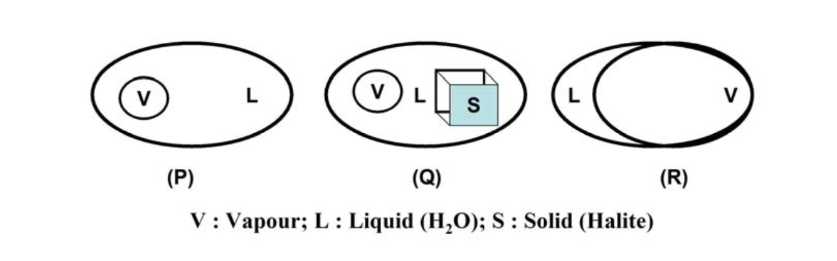
\includegraphics[width=1.0\textwidth]{figs/fig2.png}
\caption{}
\label{fig:q46_inclusions}
\end{figure}

The salinity can be determined by

\hfill{\brak{\text{GATE GG 2012}}}

\begin{multicols}{2}
\begin{enumerate}
\item heating of P, freezing of Q
\item heating of Q, freezing of R
\item freezing of P, heating of R
\item heating of all P, Q and R
\end{enumerate}
\end{multicols}

\item Study the map below showing elevation of selected locations and outcrops of sedimentary beds.

\begin{figure}[H]
\centering
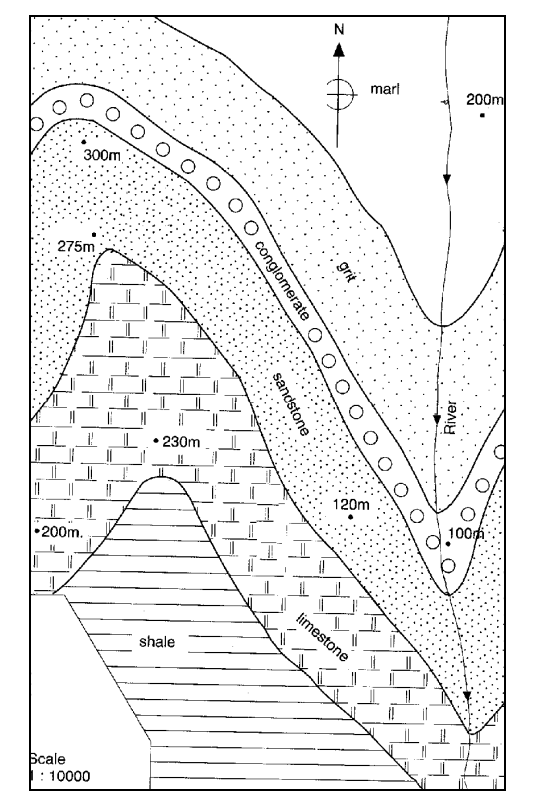
\includegraphics[width=0.75\textwidth]{figs/fig3.png}
\caption{}
\label{fig:q47_map}
\end{figure}

Which of the following statements is correct?

\hfill{\brak{\text{GATE GG 2012}}}

\begin{multicols}{2}
\begin{enumerate}
\item The beds dip easterly
\item The beds dip westerly
\item The beds dip southerly
\item The beds are folded
\end{enumerate}
\end{multicols}

\textbf{Common Data for Questions 48 and 49:}

The figures P and Q represent schematic binary phase diagrams for solid–melt and subsolidus relations in temperature (T)–composition (X) space.

\begin{figure}[H]
\centering
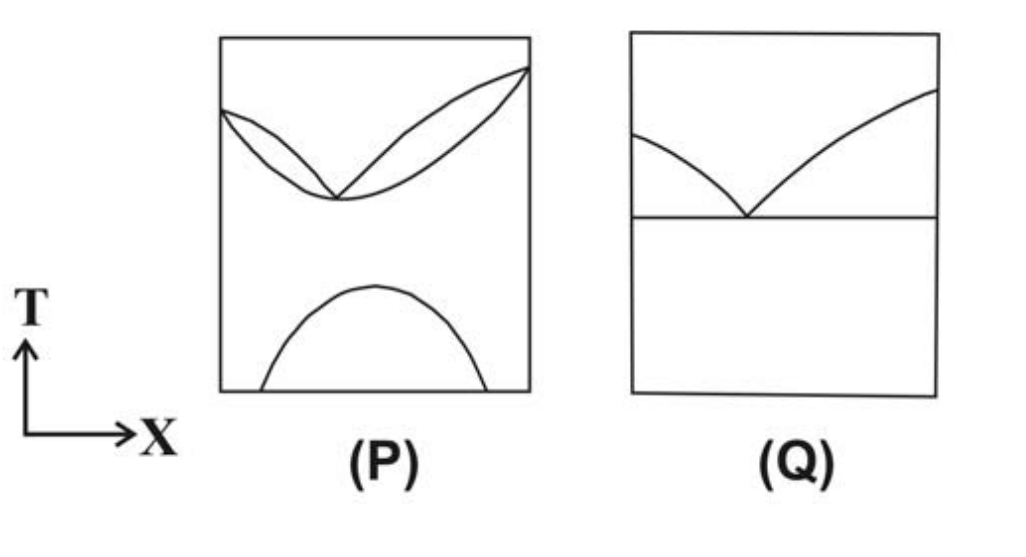
\includegraphics[width=0.9\textwidth]{figs/fig4.png}
\caption{}
\label{fig:q48_phases}
\end{figure}

\item  Which of the following statements is true?

\hfill{\brak{\text{GATE GG 2012}}}

\begin{multicols}{2}
\begin{enumerate}
\item P shows eutectic relation and Q shows high temperature limited solid solution
\item Both P and Q show high temperature limited solid solution
\item Both P and Q show eutectic relation
\item P shows high temperature limited solid solution and Q shows eutectic relation
\end{enumerate}
\end{multicols}

\item Choose the correct statement?

\hfill{\brak{\text{GATE GG 2012}}}

\begin{multicols}{2}
\begin{enumerate}
\item Solvus occurs in both P and Q
\item Solvus is absent in both P and Q
\item Solvus occurs in P but not in Q
\item Solvus occurs in Q but not in P
\end{enumerate}
\end{multicols}

\textbf{Common Data for Questions 50 and 51}\\
The following figure gives Mohr envelope for a rock and Mohr circle in a particular stress condition. Fracturing occurs when the Mohr circle touches the Mohr envelope at B.

\begin{figure}[H]
\centering
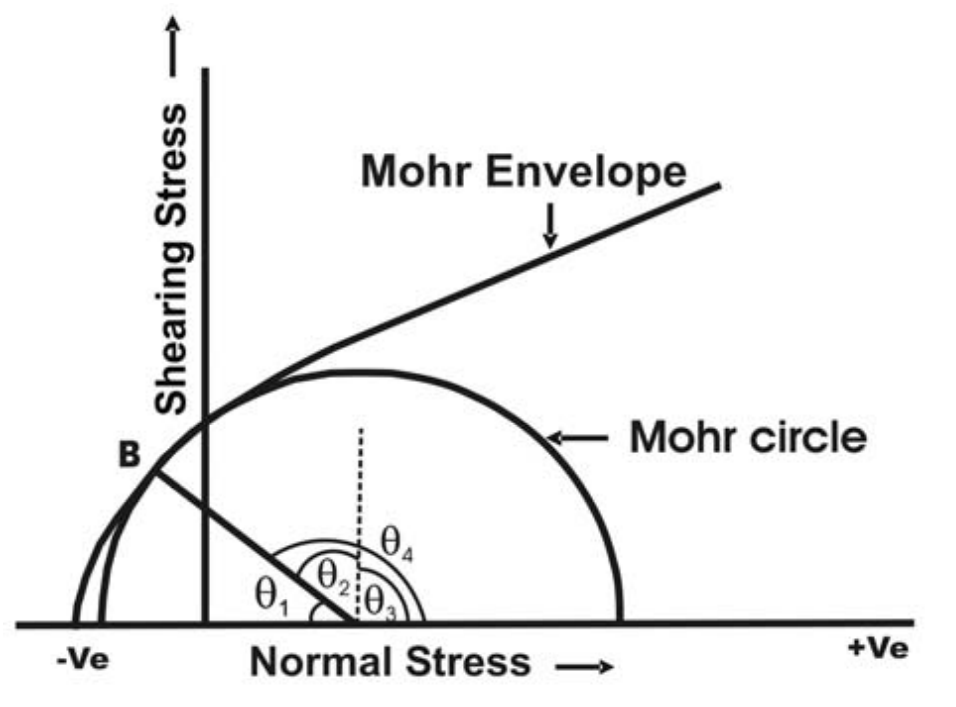
\includegraphics[width=0.6\textwidth]{figs/fig5.png}
\caption{}
\label{fig:q50_mohr}
\end{figure}

\item What type of fractures will develop in the rock?

\hfill{\brak{\text{GATE GG 2012}}}

\begin{multicols}{2}
\begin{enumerate}
\item Extension fractures
\item Conjugate shear fractures
\item Columnar fractures
\item Hybrid extension-shear fractures
\end{enumerate}
\end{multicols}

\item  What is the dihedral angle?

\hfill{\brak{\text{GATE GG 2012}}}

\begin{multicols}{4}
\begin{enumerate}
\item $\theta_1$
\item $\theta_2$
\item $\theta_3$
\item $\theta_4$
\end{enumerate}
\end{multicols}

\textbf{Linked Answer Questions}\\
\textbf{Linked Answer Questions 52 and 53:}

A thick section of clean sand is identified on a suite of geophysical logs. The deep laterolog reads 4 Ohm-m in the upper part of the section and 0.1 Ohm-m in the lower part of the section. The lower part is interpreted to be 100\% water-saturated. The resistivity of formation water obtained from SP log is estimated to be 0.01 Ohm-m.

\item  The formation resistivity factor of the clean sand section is

\hfill{\brak{\text{GATE GG 2012}}}

\begin{multicols}{4}
\begin{enumerate}
\item 8
\item 10
\item 12
\item 14
\end{enumerate}
\end{multicols}

\newpage 

\item Based on the above result, the water saturation in the top part of the sand formation is

\hfill{\brak{\text{GATE GG 2012}}}

\begin{multicols}{4}
\begin{enumerate}
\item 0.125
\item 0.158
\item 0.165
\item 0.184
\end{enumerate}
\end{multicols}

\textbf{Statement for Linked Answer Questions 54 and 55:}

Microfossils are widely used in palaeoceanographic studies.

\item Which of the following microfossil groups is generally found in deep sea below the Carbonate Compensation Depth?

\hfill{\brak{\text{GATE GG 2012}}}

\begin{multicols}{4}
\begin{enumerate}
\item Foraminifera
\item Radiolaria
\item Cocoliths
\item Ostracods
\end{enumerate}
\end{multicols}

\item What is the test composition of the microfossil group identified above?

\hfill{\brak{\text{GATE GG 2012}}}

\begin{multicols}{4}
\begin{enumerate}
\item Carbonate
\item Phosphate
\item Nitrate
\item Siliceous
\end{enumerate}
\end{multicols}
\end{enumerate}

\end{enumerate}

\begin{align*}
    {\Large{\textbf{END OF SECTION 1 OF PART B}}}
\end{align*}

\begin{align*}
    {\large{\textbf{PART B (SECTION 2) FOR GEOPHYSICS CANDIDATES ONLY}}}
\end{align*}

\begin{enumerate}
\setcounter{enumi}{25}

\item The average magnetic susceptibility of dolerite is 1400. What is its magnetic permeability in h/m? \brak{\text{Give answer up to 5 decimal places}}

\hfill{\brak{\text{GATE GG 2012}}}

\begin{multicols}{4}
\begin{enumerate}
\item 0.00176
\item 0.00211
\item 0.00302
\item 0.00354
\end{enumerate}
\end{multicols}

\item A small scale seismic reflection survey was conducted with a shot point located at the middle of a 500 m long geophone spread. The NMO-corrected travel times at the end of the spread were found to be 1.227 s and 1.255 s. If the average seismic wave velocity above the reflector is 2500 m/s, what is the dip of the reflector? \brak{\text{Give the value in degrees in nearest integer}}

\hfill{\brak{\text{GATE GG 2012}}}

\begin{multicols}{4}
\begin{enumerate}
\item 4
\item 6
\item 8
\item 10
\end{enumerate}
\end{multicols}

\item The S-wave velocity in the lower continental crust is 6800 m/s and its density is 3380 kg/m\(^3\). Find its rigidity in GPa. \brak{\text{Give answer up to 2 decimal places}}

\hfill{\brak{\text{GATE GG 2012}}}

\begin{multicols}{4}
\begin{enumerate}
\item 156.29
\item 160.21
\item 162.34
\item 164.11
\end{enumerate}
\end{multicols}

\item Given the frequency of an electromagnetic wave to be 1 kHz and ground conductivity to be 10 S/m, calculate the skin depth. \brak{\text{Give answer in nearest integer, in meters}}

\hfill{\brak{\text{GATE GG 2012}}}

\begin{multicols}{4}
\begin{enumerate}
\item 2
\item 3
\item 5
\item 8
\end{enumerate}
\end{multicols}
\newpage


\item Based on acoustic log of a well, the transit time in a water-bearing sandstone zone is found to be 75 \(\mu\)s/ft. The transit time of acoustic wave through the sandstone matrix and water are 50 \(\mu\)s/ft and 200 \(\mu\)s/ft, respectively. Determine the porosity of the sandstone. \brak{\text{Give answer up to 2 decimal places}}

\hfill{\brak{\text{GATE GG 2012}}}

\begin{multicols}{4}
\begin{enumerate}
\item 0.05
\item 0.10
\item 0.12
\item 0.17
\end{enumerate}
\end{multicols}

\item In frequency domain IP method, frequency effect is defined as

\hfill{\brak{\text{GATE GG 2012}}}

\begin{multicols}{2}
\begin{enumerate}
\item \(\dfrac{\rho_{ac}-\rho_{dc}}{\rho_{dc}}\)
\item \(\dfrac{\rho_{ac}-\rho_{dc}}{\rho_{ac}}\)
\item \(\dfrac{\rho_{dc}-\rho_{ac}}{\rho_{dc}}\)
\item \(\dfrac{\rho_{dc}-\rho_{ac}}{\rho_{ac}}\)
\end{enumerate}
\end{multicols}

\item The bright spot on a seismic reflection section in a sand–shale sequence can be seen over

\hfill{\brak{\text{GATE GG 2012}}}

\begin{multicols}{4}
\begin{enumerate}
\item fresh water-bearing sand
\item saline water-bearing sand
\item oil pool
\item gas pool
\end{enumerate}
\end{multicols}

\item The line joining the north and south magnetic dip poles misses the Earth’s centre by about \brak{\text{in km}}

\hfill{\brak{\text{GATE GG 2012}}}

\begin{multicols}{4}
\begin{enumerate}
\item 1000
\item 1100
\item 1200
\item 1300
\end{enumerate}
\end{multicols}

\item For a three-layered earth with resistivities \(\rho_1\), \(\rho_2\), and \(\rho_3\), and corresponding thicknesses \(h_1\), \(h_2\), and \(h_3\) respectively, the quantity \((h_1/\rho_1) + (h_2/\rho_2) + (h_3/\rho_3)\) stands for

\hfill{\brak{\text{GATE GG 2012}}}

\begin{multicols}{4}
\begin{enumerate}
\item longitudinal conductance
\item transverse resistance
\item apparent conductance
\item apparent resistance
\end{enumerate}
\end{multicols}

\item The distance between the centre of the Earth and the barycentre \brak{\text{i.e. centre of mass of the Earth–Moon system}} is \brak{\text{in km}}

\hfill{\brak{\text{GATE GG 2012}}}

\begin{multicols}{4}
\begin{enumerate}
\item 4510
\item 4670
\item 4810
\item 4860
\end{enumerate}
\end{multicols}

\item The change in gravity caused by Earth’s tides on the land surface in a complete tidal cycle is in the range of \brak{\text{in milligal}}

\hfill{\brak{\text{GATE GG 2012}}}

\begin{multicols}{2}
\begin{enumerate}
\item 0.1 to 0.2
\item 0.2 to 0.3
\item 0.3 to 0.4
\item 0.4 to 0.5
\end{enumerate}
\end{multicols}

\item Terrestrial heat flow is the product of

\hfill{\brak{\text{GATE GG 2012}}}


\begin{enumerate}
\item thermal diffusivity and temperature
\item thermal conductivity and temperature
\item thermal diffusivity and temperature gradient
\item thermal conductivity and temperature gradient
\end{enumerate}

\newpage


\item According to Archie's equation, the electrical resistivity of porous sandstone doesn't depend on:

\hfill{\brak{\text{GATE GG 2012}}}

\begin{multicols}{2}
\begin{enumerate}
\item porosity
\item nature of interstitial fluid
\item tortuosity of pores
\item solid matrix
\end{enumerate}
\end{multicols}

\item Match the items in Group I with those in Group II.\\
Group I \quad\qquad\qquad\qquad\qquad Group II\\
P. Magnetic susceptibility \qquad 1. Gyromagnetic ratio\\
Q. Airborne magnetic survey \quad 2. Axial dipole\\
R. Geomagnetic field \qquad\qquad 3. Diamagnetism\\
S. Proton precession magnetometer \quad 4. Total field intensity\\
\phantom{Group I} \qquad\qquad\qquad\qquad\qquad\qquad 5. Poisson's relation

\hfill{\brak{\text{GATE GG 2012}}}


\begin{enumerate}
\item P-3, Q-4, R-2, S-1
\item P-5, Q-2, R-4, S-3
\item P-1, Q-4, R-1, S-5
\item P-4, Q-3, R-3, S-1
\end{enumerate}


\item The NMO of a diffraction hyperbola as compared to that of a reflection hyperbola is

\hfill{\brak{\text{GATE GG 2012}}}

\begin{multicols}{4}
\begin{enumerate}
\item always greater
\item always smaller
\item random
\item same
\end{enumerate}
\end{multicols}

\item Which one of the following can be determined from the NMR log against sandstone?

\hfill{\brak{\text{GATE GG 2012}}}

\begin{multicols}{2}
\begin{enumerate}
\item Clay content of sandstone
\item Total porosity
\item Water-filled porosity
\item Structured water
\end{enumerate}
\end{multicols}

\item The peak in the response curves obtained from a geophone exhibits

\hfill{\brak{\text{GATE GG 2012}}}


\begin{enumerate}
\item shift to lower frequency with increasing damping coefficient
\item shift to higher frequency with increasing damping coefficient
\item no shift in frequency with increasing damping coefficient
\item increase in amplitude with increasing damping coefficient
\end{enumerate}


\item The solution to the purely under-determined problem \(Gm=d\) is given by

\hfill{\brak{\text{GATE GG 2012}}}

\begin{multicols}{1}
\begin{enumerate}
\item \((G^{T}G)^{-1}G^{T}d\)
\item \((G^{T}G)^{-1}G\,d^{T}\)
\item \(G^{T}(GG^{T})^{-1}d\)
\item \(G^{T}d\,(GG^{T})^{-1}\)
\end{enumerate}
\end{multicols}

\item Given the following matrix equation:\\
\(A_{m\times n}\,X_{x\times 1}=b_{m\times 1}\), \quad the nature of this system of equation is

\hfill{\brak{\text{GATE GG 2012}}}

\begin{multicols}{2}
\begin{enumerate}
\item over-determined if \(m>n\)
\item under-determined if \(m<n\)
\item even-determined if \(m=n\)
\item determined by the rank of the matrix \(A\)
\end{enumerate}
\end{multicols}

\newpage

\item Match the items in Group I with those in Group II.\\
Group I \quad Group II\\
P. \(10^{-4}\) to 1 Hz \quad 1. VLF\\
Q. 400 to 2000 Hz \quad 2. GPR\\
R. 20 kHz to 25 kHz \quad 3. MT\\
S. 25 MHz to 1.2 GHz \quad 4. Slingram

\hfill{\brak{\text{GATE GG 2012}}}

\begin{multicols}{1}
\begin{enumerate}
\item P-2, Q-1, R-4, S-3
\item P-3, Q-4, R-1, S-2
\item P-1, Q-4, R-3, S-2
\item P-3, Q-2, R-1, S-4
\end{enumerate}
\end{multicols}




\item Gamma-gamma log applied for estimation of formation density uses incident rays with energy in the range of 0.5 MeV to 2.0 MeV. The interaction of such gamma rays with rocks is governed by

\hfill{\brak{\text{GATE GG 2012}}}

\begin{multicols}{2}
\begin{enumerate}
\item photoelectric absorption
\item Compton scattering
\item pair production
\item secondary emission of gamma rays
\end{enumerate}
\end{multicols}

\item Determine the correctness or otherwise of the following Assertion \brak{\text{a}} and Reason \brak{\text{r}}.\\
Assertion: In a well-log survey using fresh-water drilling mud, an oil-bearing sandstone zone can be identified by electrical resistivity and SP logs.\\
Reason: Oil has high electrical resistivity and the porous nature of sandstone is indicated by negative SP.

\hfill{\brak{\text{GATE GG 2012}}}


\begin{enumerate}
\item $[a]$ is true but [r] is false
\item $[a]$ is false but [r] is true
\item both [a] and [r] are true but [r] is not the correct reason for [a]
\item both [a] and [r] are true and [r] is the correct reason for [a]
\end{enumerate}


\textbf{Common Data Questions}\\
\textbf{Common Data for Questions 48 and 49:}\\
A signal having duration of 10 seconds is sampled at a rate of 1000 samples per second. The maximum frequency of the sampled signal is 475 Hz.

\item If the signal has been under-sampled, the maximum frequency \brak{\text{in Hz}} of the original signal would have been

\hfill{\brak{\text{GATE GG 2012}}}

\begin{multicols}{4}
\begin{enumerate}
\item 475
\item 500
\item 525
\item 550
\end{enumerate}
\end{multicols}

\item What is the frequency interval \brak{\text{in Hz}} at which the spectrum of the above signal is evaluated?

\hfill{\brak{\text{GATE GG 2012}}}

\begin{multicols}{4}
\begin{enumerate}
\item 0.08
\item 0.10
\item 0.12
\item 0.14
\end{enumerate}
\end{multicols}

\textbf{Common Data for Questions 50 and 51:} \\
In a sequence of equally thick layers in the subsurface, normally incident reflection coefficients at the three interfaces are: 0.10, 0.15 and 0.18.

\item The amplitude of primary reflection from the deepest interface is

\hfill{\brak{\text{GATE GG 2012}}}

\begin{multicols}{4}
\begin{enumerate}
\item 0.184
\item 0.174
\item 0.165
\item 0.156
\end{enumerate}
\end{multicols}

\item The amplitude of the surface multiple that arrives along with the reflection from the deepest interface is

\hfill{\brak{\text{GATE GG 2012}}}

\begin{multicols}{4}
\begin{enumerate}
\item 0.008
\item 0.005
\item 0.003
\item 0.001
\end{enumerate}
\end{multicols}

\textbf{Linked Answer Questions}\\
\textbf{Statement for Linked Answer Questions 52 and 53:}\\
A thick section of clean sand is identified on a suite of geophysical logs. The deep laterolog reads 4 Ohm-m in the upper part of the section and 0.1 Ohm-m in the lower part of the section. The lower part is interpreted to be 100\% water-saturated. The resistivity of formation water obtained from SP log is estimated to be 0.01 Ohm-m.

\item The formation resistivity factor of the clean sand section is

\hfill{\brak{\text{GATE GG 2012}}}

\begin{multicols}{4}
\begin{enumerate}
\item 8
\item 10
\item 12
\item 14
\end{enumerate}
\end{multicols}

\item Based on the above result, the water saturation in the top part of the sand formation is

\hfill{\brak{\text{GATE GG 2012}}}

\begin{multicols}{4}
\begin{enumerate}
\item 0.125
\item 0.158
\item 0.165
\item 0.184
\end{enumerate}
\end{multicols}

\textbf{Statement for Linked Answer Questions 54 and 55:}\\
The seismic slip of a fault after an earthquake is measured to be 0.5 m and the fault area is estimated to be 250 km$^{2}$. The rigidity of the medium surrounding the fault is 30 GPa.

\item The seismic moment \brak{\text{in Nm}} of the earthquake is

\hfill{\brak{\text{GATE GG 2012}}}

\begin{multicols}{2}
\begin{enumerate}
\item \(3.75 \times 10^{18}\)
\item \(3.75 \times 10^{16}\)
\item \(3.75 \times 10^{14}\)
\item \(3.75 \times 10^{12}\)
\end{enumerate}
\end{multicols}

\item Based on the above, the moment magnitude of the earthquake is

\hfill{\brak{\text{GATE GG 2012}}}

\begin{multicols}{4}
\begin{enumerate}
\item 5.15
\item 5.36
\item 6.35
\item 7.25
\end{enumerate}
\end{multicols}

\begin{align*}
    {\Large{\textbf{END OF SECTION 2 OF PART B}}}
\end{align*}

\textbf{General Aptitude \brak{\text{GA}} Questions}\\
\textbf{Q. 56 -- Q. 60 carry one mark each.}



\item Which one of the following options is the closest in meaning to the word given below?

Pacify

\hfill{\brak{\text{GATE GG 2012}}}

\begin{multicols}{4}
\begin{enumerate}
\item Excite
\item Soothe
\item Deplete
\item Tire
\end{enumerate}
\end{multicols}

\item Choose the most appropriate pair of words from the options given below to complete the following sentence:

\textbf{The high level of \_\_\_ of the questions in the test was \_\_\_ by an increase in the period of time allotted for answering them.}

\hfill{\brak{\text{GATE GG 2012}}}

\begin{multicols}{2}
\begin{enumerate}
\item difficulty, compensated
\item exactitude, magnified
\item aptitude, decreased
\item attitude, mitigated
\end{enumerate}
\end{multicols}

\item Choose the grammatically \textbf{CORRECT} sentence:

\hfill{\brak{\text{GATE GG 2012}}}

\begin{multicols}{1}
\begin{enumerate}
\item He laid in bed till 8 o’clock in the morning.
\item He layed in bed till 8 o’clock in the morning.
\item He lain in bed till 8 o’clock in the morning.
\item He lay in bed till 8 o’clock in the morning.
\end{enumerate}
\end{multicols}

\item Which one of the parts \brak{\text{A, B, C, D}} in the sentence contains an ERROR?

\textbf{No sooner had the doctor seen the results of the blood test, than he suggested the patient to see the specialist.}

\hfill{\brak{\text{GATE GG 2012}}}

\begin{multicols}{2}
\begin{enumerate}
\item no sooner had
\item results of the blood test
\item suggested the patient
\item see the specialist
\end{enumerate}
\end{multicols}

\item Ten teams participate in a tournament. Every team plays each of the other teams twice. The total number of matches to be played is

\hfill{\brak{\text{GATE GG 2012}}}

\begin{multicols}{4}
\begin{enumerate}
\item 20
\item 45
\item 60
\item 90
\end{enumerate}
\end{multicols}

\textbf{ Q. 61 -- Q. 65 carry two marks each.}

\item A value of $x$ that satisfies the equation $\log x + \log \brak{\text{$x - 7$}} = \log \brak{\text{$x + 11$}} + \log 2$ is

\hfill{\brak{\text{GATE GG 2012}}}

\begin{multicols}{4}
\begin{enumerate}
\item 1
\item 2
\item 7
\item 11
\end{enumerate}
\end{multicols}

\item Let $f(x) = x - [x]$, where $x \ge 0$ and $[x]$ is the greatest integer not larger than $x$. Then $f(x)$ is a

\hfill{\brak{\text{GATE GG 2012}}}

\begin{multicols}{2}
\begin{enumerate}
\item monotonically increasing function
\item monotonically decreasing function
\item linearly increasing function between two integers
\item linearly decreasing function between two integers
\end{enumerate}
\end{multicols}

\item Ravi is taller than Arun but shorter than Iqbal. Sam is shorter than Ravi. Mohan is shorter than Arun. Balu is taller than Mohan and Sam. The tallest person can be

\hfill{\brak{\text{GATE GG 2012}}}

\begin{multicols}{4}
\begin{enumerate}
\item Mohan
\item Ravi
\item Balu
\item Arun
\end{enumerate}
\end{multicols}

\item A smuggler has 10 capsules in which five are filled with narcotic drugs and the rest contain the original medicine. All the 10 capsules are mixed in a single box, from which the customs officials picked two capsules at random and tested for the presence of narcotic drugs. The probability that the smuggler will be caught is

\hfill{\brak{\text{GATE GG 2012}}}

\begin{multicols}{4}
\begin{enumerate}
\item 0.50
\item 0.67
\item 0.78
\item 0.82
\end{enumerate}
\end{multicols}

\newpage

\item The documents expose the cynicism of the government officials – and yet as the media website reflects, not a single newspaper has reported on their existence.

Which one of the following inferences may be drawn with the greatest accuracy from the above passage?

\hfill{\brak{\text{GATE GG 2012}}}

\begin{enumerate}
\item Nobody other than the government officials knew about the existence of the documents.
\item Newspapers did report about the documents but nobody cared.
\item Media reports did not show the existence of the documents.
\item The documents reveal the attitude of the government officials.
\end{enumerate}


















\end{enumerate}



\begin{align*}
    {\Large{\textbf{END OF THE QUESTION PAPER}}}
\end{align*}














\end{document}